\immediate\write18{tex penrose.dtx}
\documentclass{article}
\usepackage[scale=.91]{geometry}
\usepackage[svgnames]{xcolor}
\usepackage{tikz}
\usetikzlibrary{penrose}
%
% 81 thin rhombi, 147 thick rhombi
%
\thispagestyle{empty}
\pagestyle{empty}
\pgfmathsetmacro\cphi{(sqrt(5)+1)/2}
\pgfmathsetmacro\sphi{sin(36)}
\pgfmathsetmacro\chphi{2*cos(18)}
\pgfmathsetmacro\shphi{sin(18)}
\colorlet{thinRhombus}{DarkOrchid}
\colorlet{thickRhombus}{DarkSlateGray}
\colorlet{circleArc}{RosyBrown}
\colorlet{longArc}{LawnGreen}

\colorlet{kite}{HotPink}
\colorlet{dart}{Fuchsia}

\colorlet{goldenTriangle}{Gold}
\colorlet{reverseGoldenTriangle}{Magenta}
\colorlet{goldenGnomon}{Cyan}
\colorlet{reverseGoldenGnomon}{LimeGreen}

\makeatletter
\tikzset{
  tint fill colour/.code={%
    \edef\@temp{%
      \def\noexpand\tikz@fillcolor{\tikz@fillcolor!#1}%
      \noexpand\tikz@addoption{\noexpand\pgfsetfillcolor{\tikz@fillcolor!#1}}%
    }%
    \@temp
  }
}
\makeatother

\begin{document}
\begin{tikzpicture}
\path[save Penrose path=a] (0,0) to[out=-30,in=100] (1,0);
\path[save Penrose path=b] (0,0) to[out=0,in=140] (1,0);
\path[save Penrose path=c] (0,0) to[out=-40,in=140] (1,0);
\MakePenroseTile{thin rhombus}
\MakePenroseTile{thick rhombus}
\MakePenroseTile{golden triangle}
\MakePenroseTile{reverse golden triangle}
\MakePenroseTile{golden gnomon}
\MakePenroseTile{reverse golden gnomon}
\MakePenroseTile{kite}
\MakePenroseTile{dart}
\end{tikzpicture}
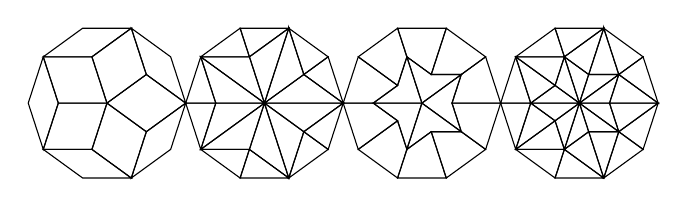
\begin{tikzpicture}[
  every Penrose tile/.style={draw},
  Penrose tile 1/.style={fill=yellow},
%  Penrose tile/.code 2 args={
%    \pgfmathsetmacro\tint{#1*20}
%    \pgfkeysalso{fill=black!\tint}
%  }
]
\foreach \tp/\pos in {rhombus/0cm,rtriangle/2cm,kite/4cm,ktriangle/6cm}
{
\begin{scope}[xshift=\pos]
\foreach[evaluate=\k as \mk using {\k+Mod(\k,2)},evaluate=\k as \ax using {Mod(\k,2) == 0 ? "T" : "t"}] \k in {0,...,9} {
  \begin{scope}[rotate=\mk*36]
  \PenroseDecomposition{\tp}{1}{\ax}
  \end{scope}
}
\end{scope}
}
\end{tikzpicture}

\begin{center}
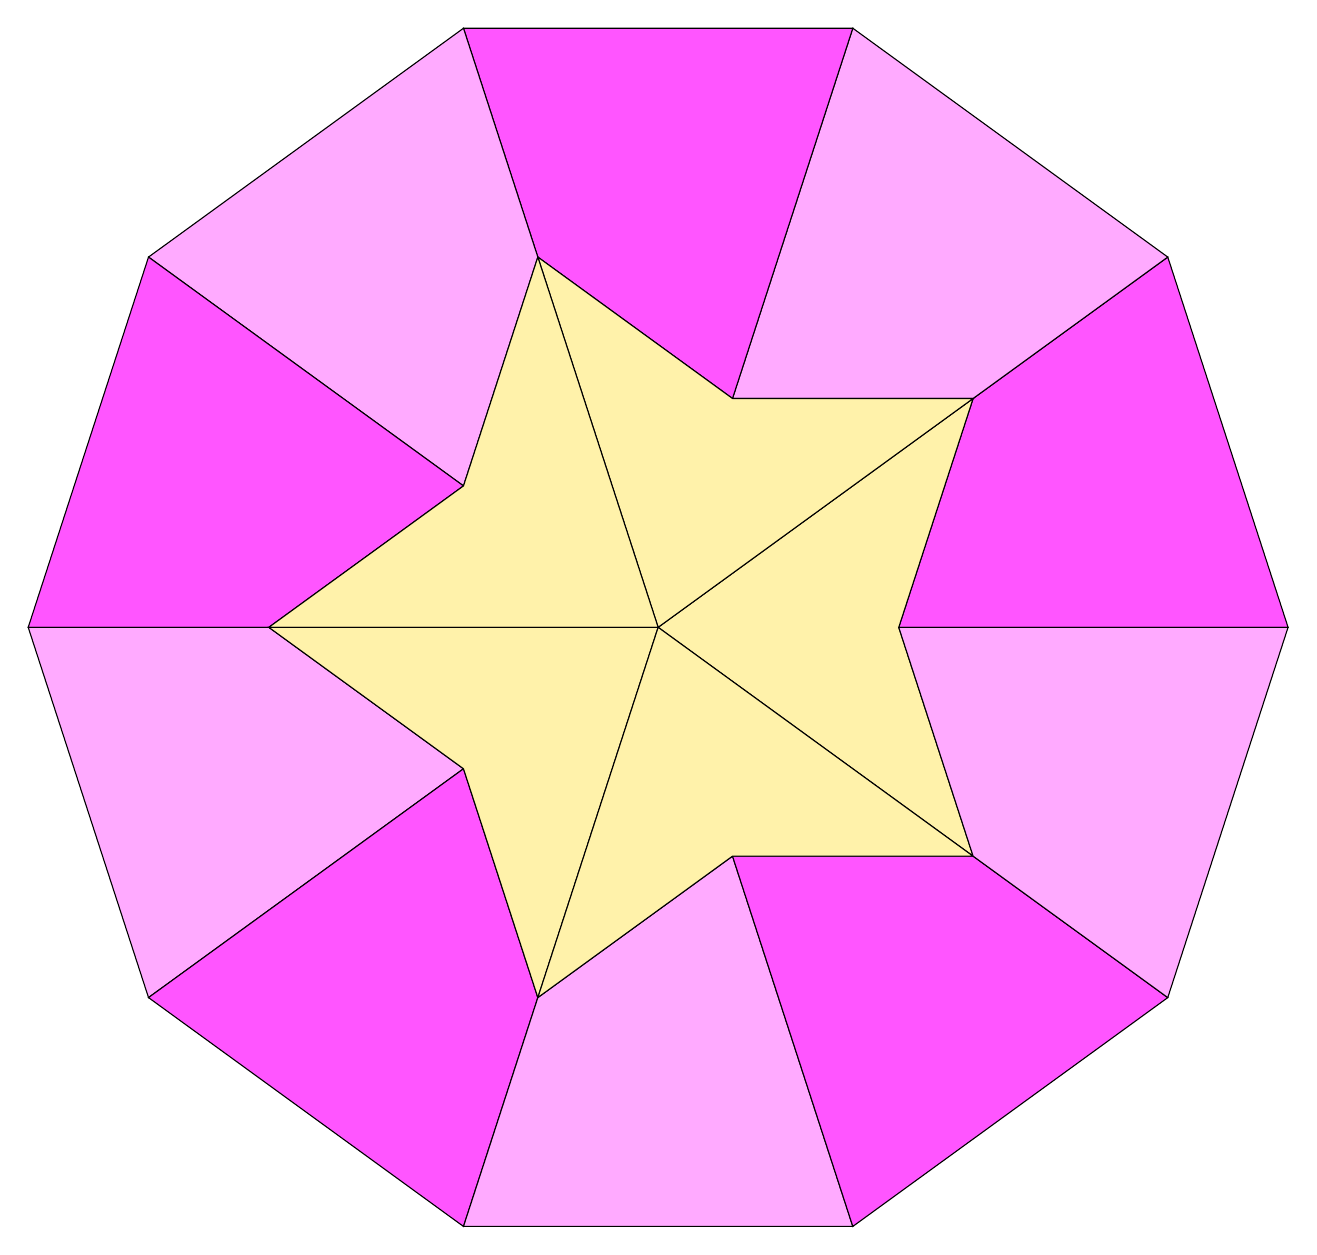
\begin{tikzpicture}[
  every Penrose tile/.style={draw},
  every golden triangle/.style={fill=goldenTriangle},
  every reverse golden triangle/.style={fill=reverseGoldenTriangle},
  every golden gnomon/.style={fill=goldenGnomon},
  every reverse golden gnomon/.style={fill=reverseGoldenGnomon},
  every kite/.style={fill=reverseGoldenTriangle},
  every dart/.style={fill=goldenTriangle},
  Penrose tile/.code 2 args={
    \pgfmathsetmacro\tint{100*(1 - #1/(1.5*#2))}
    \pgfkeysalso{tint fill colour=\tint}
%    \message{#1 and #2,}
  }
]
\foreach[evaluate=\k as \mk using {\k+Mod(\k,2)},evaluate=\k as \ax using {Mod(\k,2) == 0 ? "T" : "t"}] \k in {0,...,9} {
  \begin{scope}[rotate=\mk*36]
  \PenroseDecomposition[Penrose step=8cm]{kite}{1}{\ax}
  \end{scope}
}
\end{tikzpicture}
\end{center}

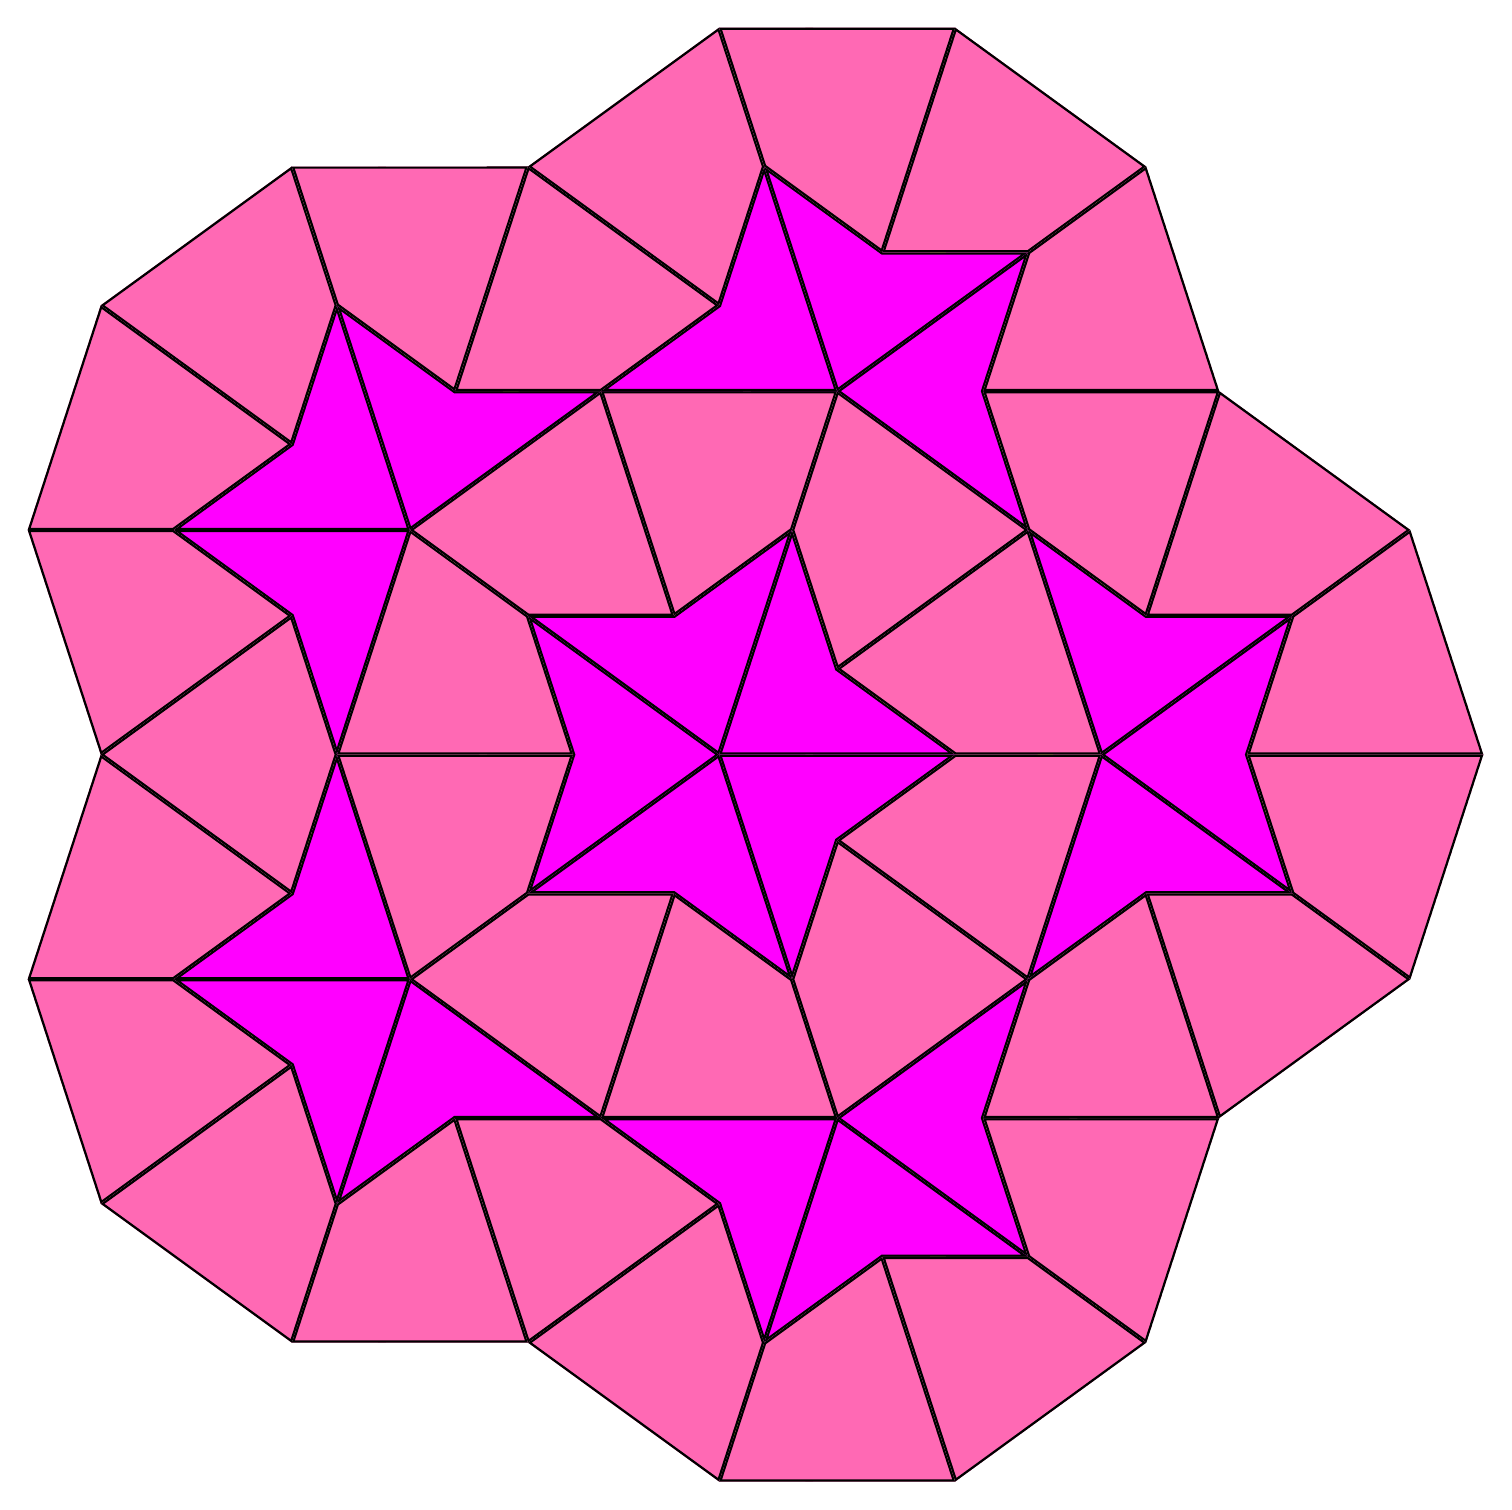
\begin{tikzpicture}[
  scale=3,
  every Penrose pic/.style={
    transform shape,
    draw=black,
    ultra thick,
  },
  every kite/.style={
    fill=kite,
  },
  every dart/.style={
    fill=dart,
  },
  every circle arc/.style={
    line width=1mm,
    draw=circleArc
  },
  every long arc/.style={
    line width=2mm,
    draw=longArc
  }
]
\pic[dart,name=a0];
\foreach[evaluate=\k as \kmo using int(\k-1)] \k in {1,...,4} {
  \pic[dart,name=a\k,align with={a\kmo} along a];
}
\foreach \k in {0,...,4} {
  \foreach \l/\e/\ee in {0/c/a,1/C/A} {
    \pic[kite,name=b\l\k,align with={a\k} along \e];
    \pic[dart,name=c\l\k,align with={b\l\k} along \ee];
    \pic[kite,name=d\l\k,align with={c\l\k} along \e];
  }
  \pic[kite,name=e\k,align with={c0\k} along C];
  \pic[dart,name=f\k,align with={c0\k} along a];
  \foreach \e in {c,C} {
    \pic[kite,name=g\k,align with={f\k} along \e];
  }
}
%\pic[dart,name=b,align with=a along c];
%\pic[kite,name=c,align with=b along c];
\end{tikzpicture}




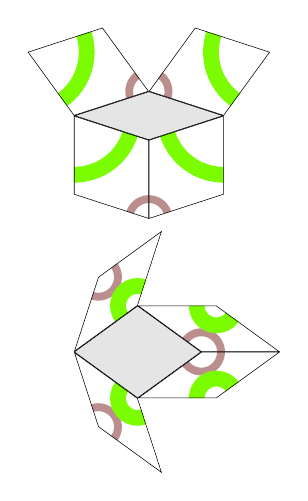
\begin{tikzpicture}[
  every circle arc/.style={
    line width=1mm,
    draw=circleArc
  },
  every long arc/.style={
    line width=2mm,
    draw=longArc
  }
]
\pic[thin rhombus,draw,name=a,fill=gray!20];
\pic[thick rhombus,draw,align with=a along a];
\pic[thick rhombus,draw,align with=a along b];
\pic[thick rhombus,draw,align with=a along A];
\pic[thick rhombus,draw,align with=a along B];
\pic[yshift=-3cm, thick rhombus,draw,name=b,fill=gray!20];
\pic[thin rhombus,draw,align with=b along a];
\pic[thin rhombus,draw,align with=b along b];
\pic[thin rhombus,draw,align with=b along A];
\pic[thin rhombus,draw,align with=b along B];
\end{tikzpicture}

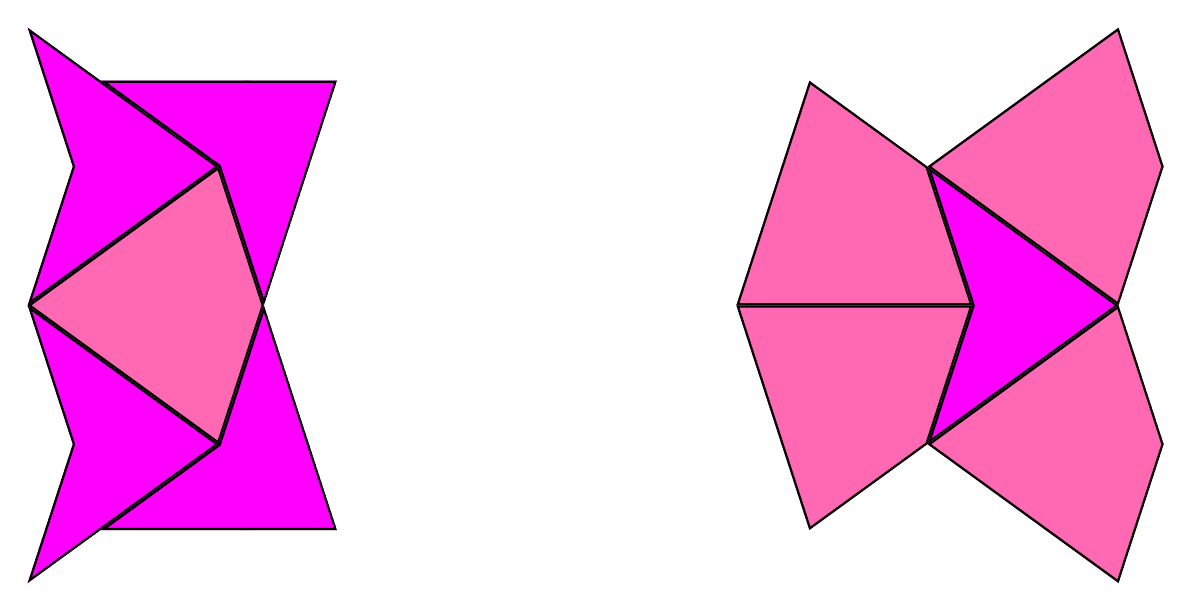
\begin{tikzpicture}[
  scale=3,
  every Penrose pic/.style={
    transform shape,
  },
  every kite/.style={
    draw=black,
    ultra thick,
    fill=kite,
  },
  every dart/.style={
    draw=black,
    ultra thick,
    fill=dart,
  },
  every circle arc/.style={
    line width=1mm,
    draw=circleArc
  },
  every long arc/.style={
    line width=2mm,
    draw=longArc
  }
]
\pic[kite,name=a,fill=gray!20];
\pic[dart,align with=a along a];
\pic[dart,align with=a along A];
\pic[dart,align with=a along c];
\pic[dart,align with=a along C];
\begin{scope}[xshift=4cm]
\pic[dart,name=a,fill=gray!20];
\pic[kite,align with=a along a];
\pic[kite,align with=a along A];
\pic[kite,align with=a along c];
\pic[kite,align with=a along C];
\end{scope}
\end{tikzpicture}



\foreach \ax in {T,t,G,g} {

\begin{tikzpicture}
\foreach \tp/\pos in {rhombus/0cm,rtriangle/2cm,kite/4cm,ktriangle/6cm}
{
\begin{scope}[xshift=\pos]
  \PenroseDecomposition[every path/.style={draw=red,ultra thick}]{\tp}{0}{\ax}
  \PenroseDecomposition[every path/.style={fill=gray!50,fill opacity=.5,draw=black}]{\tp}{1}{\ax}
\end{scope}
}
\end{tikzpicture}

}

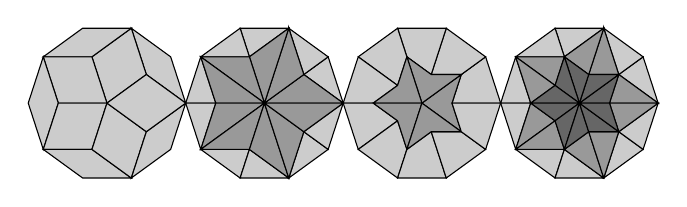
\begin{tikzpicture}[
  every Penrose tile/.style={draw},
  Penrose tile 1/.style={fill=yellow},
  Penrose tile/.code 2 args={
    \pgfmathsetmacro\tint{#1*20}
    \pgfkeysalso{fill=black!\tint}
  }
]
\foreach \tp/\pos in {rhombus/0cm,rtriangle/2cm,kite/4cm,ktriangle/6cm}
{
\begin{scope}[xshift=\pos]
\foreach[evaluate=\k as \mk using {\k+Mod(\k,2)},evaluate=\k as \ax using {Mod(\k,2) == 0 ? "T" : "t"}] \k in {0,...,9} {
  \begin{scope}[rotate=\mk*36]
  \PenroseDecomposition{\tp}{1}{\ax}
  \end{scope}
}
\end{scope}
}
\end{tikzpicture}


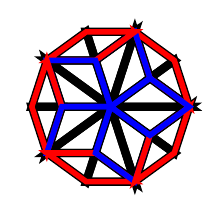
\begin{tikzpicture}[
  every Penrose tile/.style={draw,line width=3pt},
  every thin rhombus/.style={draw=red,line width=2pt},
  every thick rhombus/.style={draw=blue,line width=2pt},
  every kite/.style={draw=none,line width=1pt},
  every dart/.style={draw=none,line width=1pt},
]
\foreach[evaluate=\k as \mk using {\k+Mod(\k,2)},evaluate=\k as \ax using {Mod(\k,2) == 0 ? "T" : "t"}] \k in {0,...,9} {
  \begin{scope}[rotate=\mk*36]
  \PenroseDecomposition{rtriangle}{1}{\ax}
  \end{scope}
}
\foreach[evaluate=\k as \mk using {\k+Mod(\k,2)},evaluate=\k as \ax using {Mod(\k,2) == 0 ? "T" : "t"}] \k in {0,...,9} {
  \begin{scope}[rotate=\mk*36]
  \PenroseDecomposition{rhombus}{1}{\ax}
  \end{scope}
}
\foreach[evaluate=\k as \mk using {\k+Mod(\k,2)},evaluate=\k as \ax using {Mod(\k,2) == 0 ? "T" : "t"}] \k in {0,...,9} {
  \begin{scope}[rotate=\mk*36]
  \PenroseDecomposition{kite}{1}{\ax}
  \end{scope}
}
\end{tikzpicture}

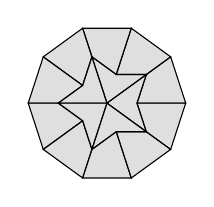
\begin{tikzpicture}[
  every Penrose tile/.style={draw,fill=gray!50, fill opacity=.5},
]
\foreach[evaluate=\k as \mk using {\k+Mod(\k,2)},evaluate=\k as \ax using {Mod(\k,2) == 0 ? "T" : "t"}] \k in {0,...,9} {
  \begin{scope}[rotate=\mk*36]
  \PenroseDecomposition{kite}{1}{\ax}
  \end{scope}
}
\end{tikzpicture}

\begin{tikzpicture}
\pic[draw,thin rhombus,at={(0,0)}];
\pic[draw,thick rhombus,at={(2,0)}];
\pic[draw,golden triangle,at={(0,-2)}];
\pic[draw,reverse golden triangle,at={(2,-2)}];
\pic[draw,golden gnomon,at={(0,-4)}];
\pic[draw,reverse golden gnomon,at={(2,-4)}];
\end{tikzpicture}

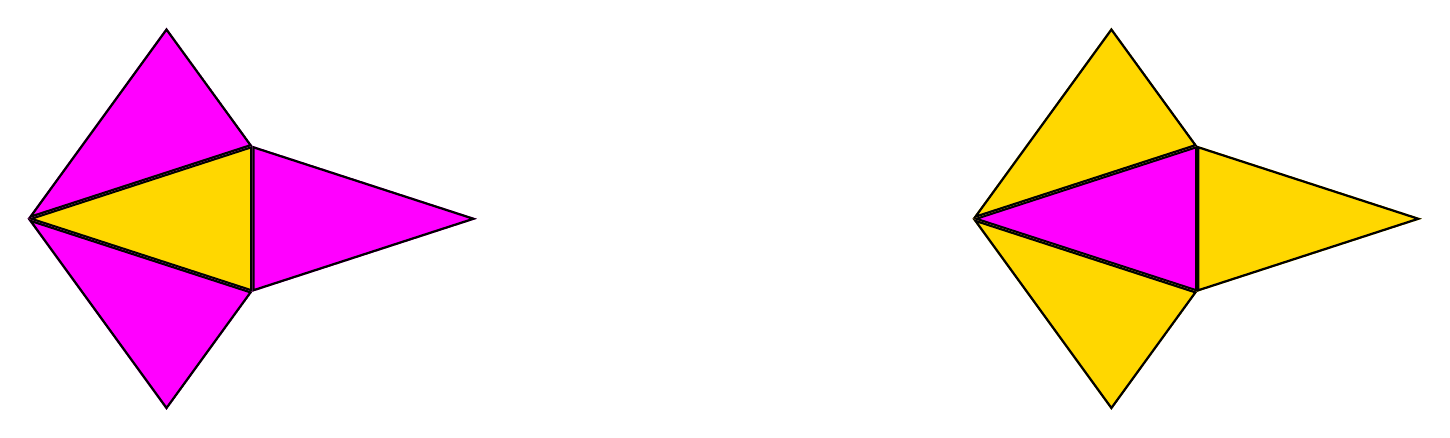
\begin{tikzpicture}[
  scale=3,
  every Penrose pic/.style={
    transform shape,
  },
  every golden triangle/.style={
    draw=black,
    ultra thick,
    fill=goldenTriangle,
  },
  every reverse golden triangle/.style={
    draw=black,
    ultra thick,
    fill=reverseGoldenTriangle,
  },
]
\pic[golden triangle,name=a];
\pic[reverse golden triangle,align with=a along a];
\pic[reverse golden triangle,align with=a along b];
\pic[reverse golden triangle,align with=a along c];
\begin{scope}[xshift=4cm]
\pic[reverse golden triangle,name=a];
\pic[golden triangle,align with=a along A];
\pic[golden triangle,align with=a along B];
\pic[golden triangle,align with=a along C];
\end{scope}
\end{tikzpicture}

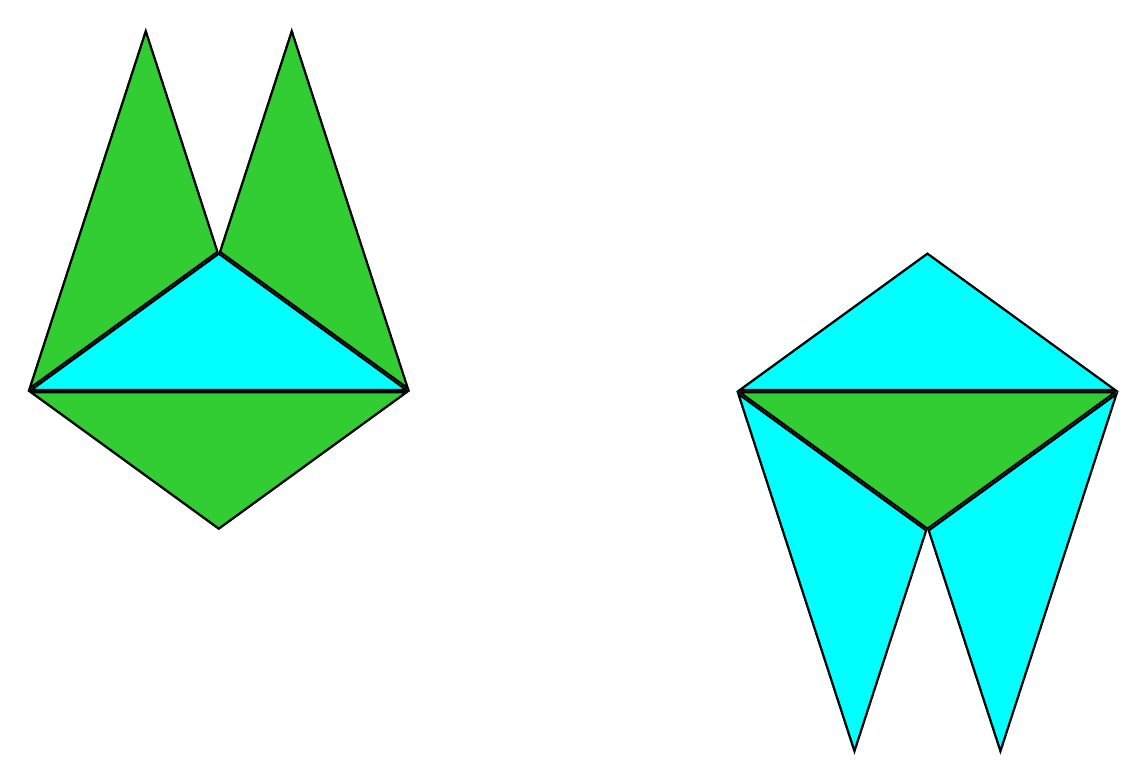
\begin{tikzpicture}[
  scale=3,
  every Penrose pic/.style={
    transform shape,
  },
  every golden gnomon/.style={
    draw=black,
    ultra thick,
    fill=goldenGnomon,
  },
  every reverse golden gnomon/.style={
    draw=black,
    ultra thick,
    fill=reverseGoldenGnomon,
  },
]
\pic[golden gnomon,name=a];
\pic[reverse golden gnomon,align with=a along C];
\pic[reverse golden gnomon,align with=a along b];
\pic[reverse golden gnomon,align with=a along A];
\begin{scope}[xshift=3cm]
\pic[reverse golden gnomon,name=a];
\pic[golden gnomon,align with=a along c];
\pic[golden gnomon,align with=a along B];
\pic[golden gnomon,align with=a along a];
\end{scope}
\end{tikzpicture}


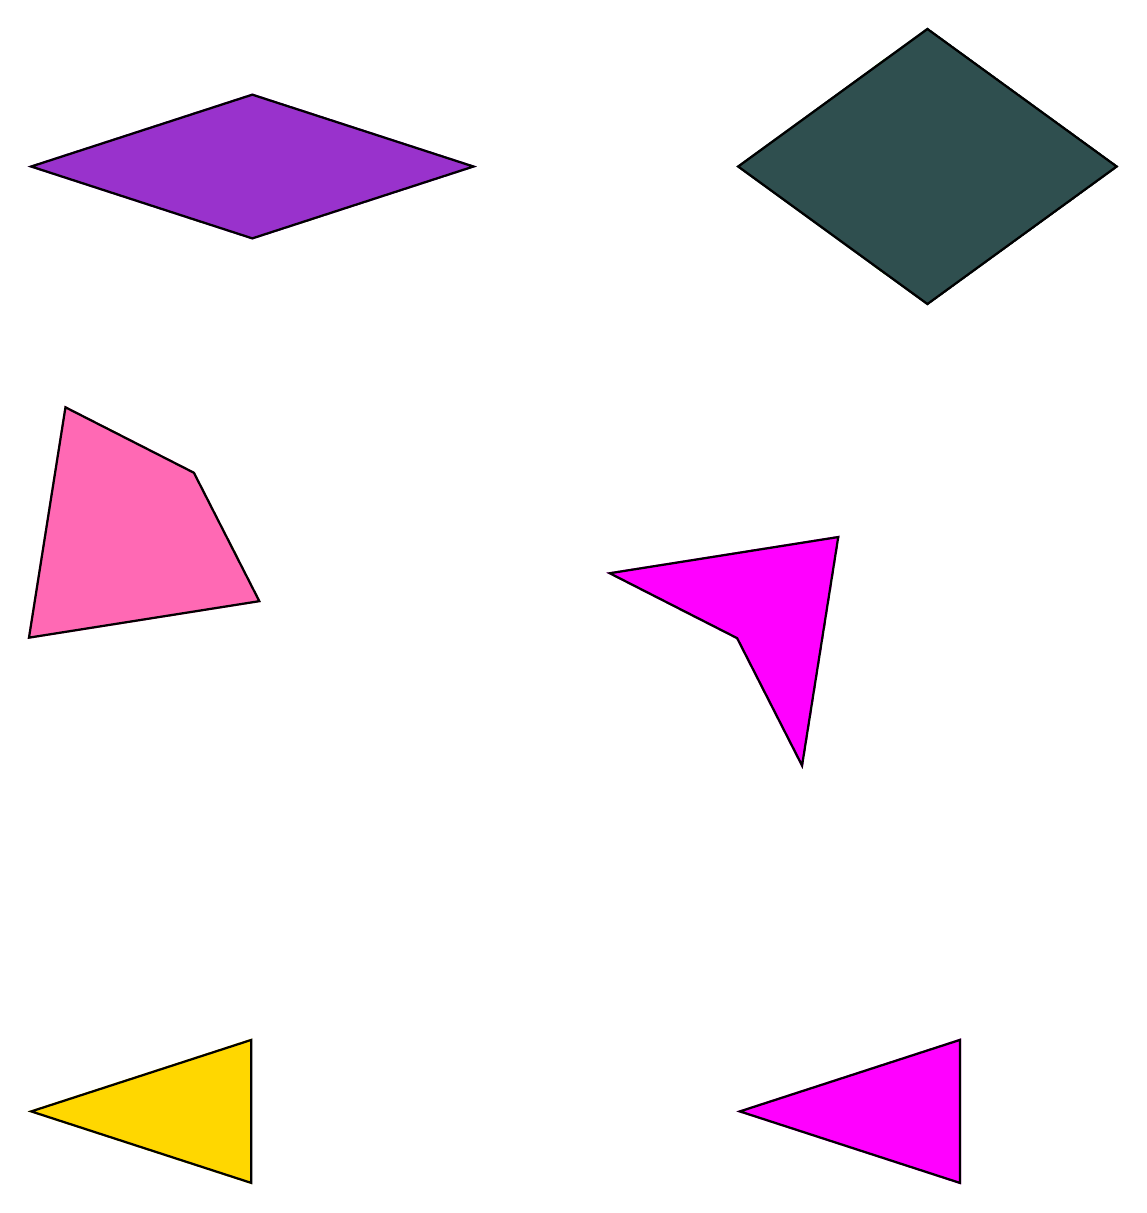
\begin{tikzpicture}[
  scale=3,
  every Penrose pic/.style={
    transform shape,
    draw=black,
    ultra thick,
  },
  every kite/.style={
    fill=kite,
  },
  every dart/.style={
    fill=dart,
  },
  every thin rhombus/.style={
    fill=thinRhombus
  },
  every thick rhombus/.style={
    fill=thickRhombus
  },
  every golden triangle/.style={
    fill=goldenTriangle
  },
  every reverse golden triangle/.style={
    fill=reverseGoldenTriangle
  },
  every circle arc/.style={
    line width=1mm,
    draw=circleArc
  },
  every long arc/.style={
    line width=2mm,
    draw=longArc
  }
]
\pic[thin rhombus];
\begin{scope}[xshift=3cm]
\pic[thick rhombus];
\end{scope}
\begin{scope}[yshift=-2cm]
\pic[rotate=45,kite];
\begin{scope}[xshift=3cm]
\pic[rotate=45,dart];
\end{scope}
\begin{scope}[yshift=-2cm]
\pic[golden triangle];
\begin{scope}[xshift=3cm]
\pic[reverse golden triangle];
\end{scope}
\end{scope}
\end{scope}
\end{tikzpicture}




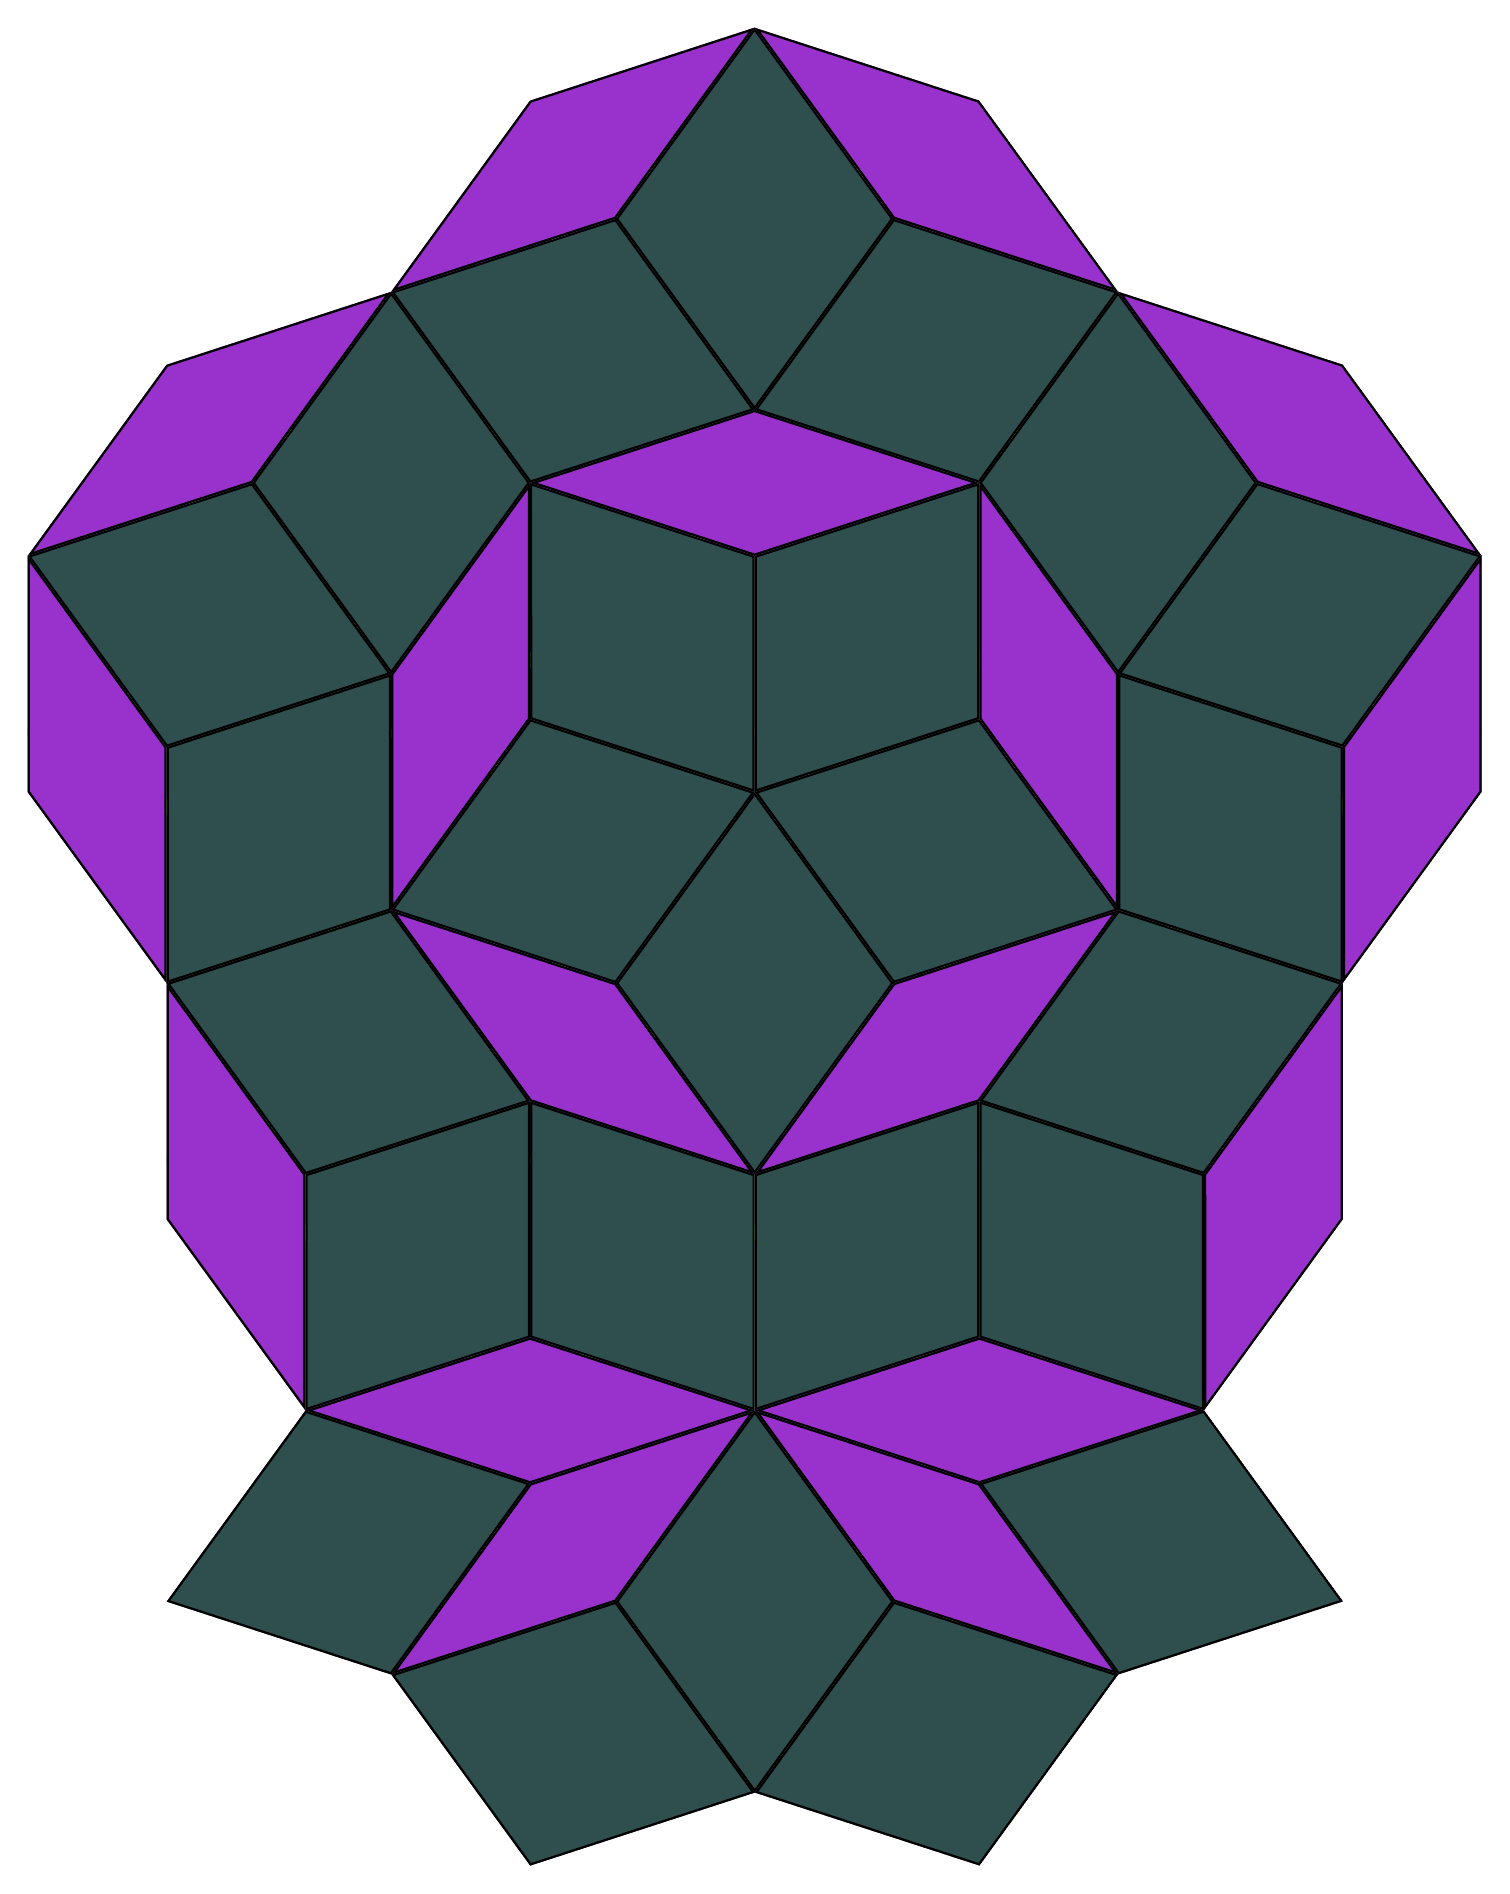
\begin{tikzpicture}[
  scale=3,
  rotate=18,
  every Penrose pic/.style={
    transform shape,
  },
  every rhombus/.style={
    draw=black,
    ultra thick,
  },
  every thin rhombus/.style={
    every rhombus/.try,
    fill=thinRhombus,
  },
  every thick rhombus/.style={
    every rhombus/.try,
    fill=thickRhombus,
  },
  every circle arc/.style={
    line width=1mm,
    draw=circleArc
  },
  every long arc/.style={
    line width=2mm,
    draw=longArc
  }
]
\pic[thick rhombus,name=a0];
\foreach[evaluate=\k as \kmo using int(\k-1)] \k in {1,...,4} 
{
  \pic[thick rhombus,name=a\k,align with={a\kmo} along A];
}
\foreach \k in {0,...,4} 
{
  \pic[thin rhombus,name=b\k,align with={a\k} along B];
  \pic[thick rhombus,name=c\k,align with={b\k} along A];
  \pic[thick rhombus,name=d\k,align with={b\k} along a];
  \pic[thick rhombus,name=e\k,align with={c\k} along A];
  \foreach \l/\a in {{0/b},{1/B}}
    \pic[thin rhombus,name=f\k\l,align with={e\k} along \a];
}
\pic[thin rhombus,name=g0,align with={f10} along a];
\pic[thin rhombus,name=g1,align with={f21} along A];
\foreach \l/\a in {{0/a},{1/A}}
  \pic[thick rhombus,name=h\l,align with={g\l} along \a];
\pic[thick rhombus,name=i,align with=g0 along B];
\foreach \l/\a in {{0/a},{1/A}}
  \pic[thick rhombus,name=j\l,align with=i along \a];
\end{tikzpicture}


\end{document}

% Local Variables:
% tex-output-type: "pdf18"
% End: